\subsection{Energy Harvesting}
Since the the Screen should be self-sufficient, some sort of Energy-Harvesting unit is needed.
It was obvious to choose light as the energy source.
A power management chip converts the energy  obtained by solar cells to a suitable voltage.
This way, a super-capacitor, which is used as an energy storage device is charged.

\subsubsection{Solar cell}
The AM-1522 by Panasonic was chosen as the solar cell.
One panel has a area of 55.0mm $\times$ 40.5mm and delivers up to 58.7$\mu\text{A}$ when operating at an optimal voltage of 2.1V.
To keep a reasonable Display to Panel ratio, four cells where used, which corresponds to an area of ca. 89.1cm (Display area = ). 


\subsubsection{Power management}

\subsubsection{Supercab}

\subsubsection{Combined test}

\begin{figure}[h]
	\centering
	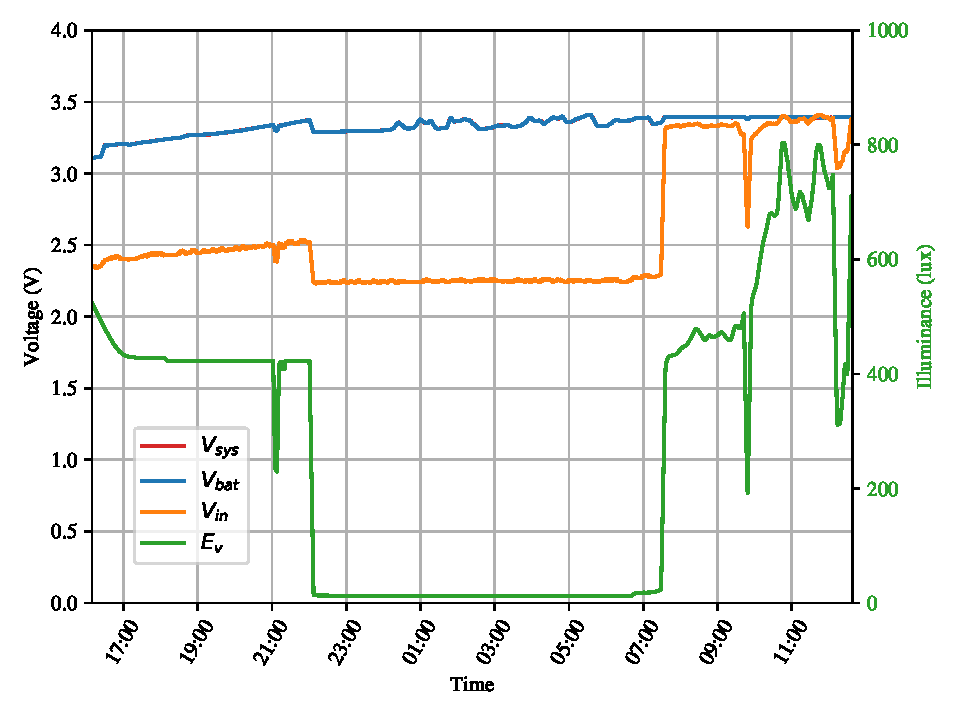
\includegraphics[width=0.9\textwidth]{4-development/hardware/graphics/laden.pdf}
	\caption{Charging behaviour\label{development:charge}}
\end{figure}

\begin{figure}[h]
	\centering
	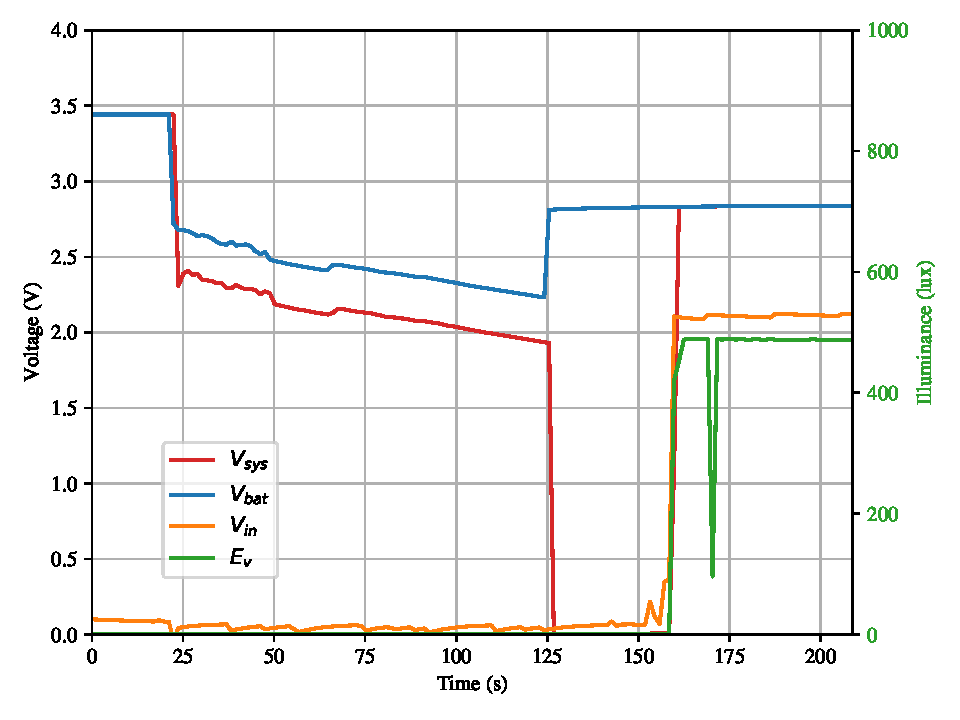
\includegraphics[width=0.9\textwidth]{4-development/hardware/graphics/entladen.pdf}
	\caption{Discharging behaviour\label{development:discharge}}
\end{figure}